\documentclass{report}
\usepackage{setspace}
\usepackage{graphicx} % Required for inserting images
\usepackage{caption}
\usepackage{subcaption}
\usepackage{amsmath} 
\usepackage[toc,page]{appendix}
\usepackage{adjustbox}
\usepackage{listings}
\usepackage{pgfplots}
\usepackage{makecell}
\usepackage{csvsimple}
\usepackage{physics}
\usepackage{cleveref}
\usepackage[dvipsnames]{xcolor}
%\definecolor{deepgray}{rgb}{.3,.3,.3}
\definecolor{deepblue}{rgb}{0,0,0.5}
\definecolor{deepred}{rgb}{0.6,0,0}
\definecolor{deepgreen}{rgb}{0,0.5,0}
\definecolor{foamC}{rgb}{0,1,1}
\lstset{frame=tb,
        numbers=left,
        basicstyle=\footnotesize\ttfamily,
        keywordstyle=\color{deepblue}\bfseries\ttfamily,
        stringstyle=\color{deepred}\ttfamily,
        commentstyle=\color{deepgreen},%\itshape\ttfamily,
        morecomment=[l][\color{magenta}]{\#},
        showstringspaces=false,
        breaklines=true,
        emphstyle=\bfseries\ttfamily}

\graphicspath{{Figures/}}

\usepackage[		% use biblatex for bibliography
backend=biber,      % use biber or bibtex backend
style=authoryear,   % choose style
natbib=true,		% allow natbib commands
hyperref=true,	    % activate hyperref support
alldates=year,      % only show year (not month)
]{biblatex}

\addbibresource{hw1writeup.bib}


\renewcommand{\chaptername}{Problem}

\title{Homework 1}
\author{Abbie Brunner}
%\date{February 22, 2024}

\onehalfspacing
\begin{document}

\maketitle

\tableofcontents

\chapter{Greens Function Validation}
We were asked to prove that $G = \frac{\ln(r)}{2\pi}$ is a valid Greens function.
There are two properties that need to be satisfied being

\begin{equation*}
   \nabla^2G = 0, \qquad \text{and} \qquad \lim_{r \to 0}\iint\nabla^2G\dd{\vb{x}} = \lim_{r \to 0}\iint \delta(\vb{y}- \vb{x}) = 1
\end{equation*}

Proving the first condition is fairly straightforward:
\begin{equation*}
   \begin{split}
      \nabla^2 G &=\pdv[2]{G}{r} + \frac{1}{r}\pdv{G}{r} + \frac{1}{r^2}\pdv[2]{G}{\theta}; \quad r=(y_i-x_i)(y_i-x_i) \\
      &= \pdv[2]{r}\qty(\frac{\ln(r)}{2\pi}) + \frac{1}{r}\pdv{r}\qty(\frac{\ln(r)}{2\pi}) + \frac{1}{r^2}\pdv[2]{\theta}\qty(\frac{\ln(r)}{2\pi}) \\
      &= \pdv{r}\qty(\frac{1}{2\pi r}) + \frac{1}{r}\qty(\frac{1}{2\pi r}) + 0 \\
      &= -\frac{1}{2\pi r^2} + \frac{1}{2\pi r^2} \\
      &= 0
   \end{split}
\end{equation*}

The second condition requires the use of Stokes' theorem.
Transforming this into a path integral allows us to simplify the integral and solve proving that the second condition is satisfied.

\begin{equation*}
   \begin{split}
      \iint \nabla^2 G \dd{\vb{x}} &= \oint \nabla G \cdot \vb{\hat{n}} \dd{S}\\
      &= \oint \pdv{G}{r}r \dd{\theta}\\
      &= \int_0^{2\pi} \frac{r}{2\pi r} \\
      &= \frac{1}{2\pi}\int_0^{2\pi}\dd{\theta} \\
      &= 1
   \end{split}
\end{equation*}

\chapter{Boundary Element Implementation}

The condition presented here is uniform flow around an object.
Using the Green's function from the last portion to solve the 2D Laplace equation we solve for the Streamfunction that makes up the $\psi_1$ portion of the combined $\psi$.
We can use the boundary condition at the surface of $\psi = 0$ and thus $\psi_1 = -\psi_0$ to evaluate $\Psi$ at each panel from the matrix approximation of
\begin{equation*}
   \frac{1}{2}\psi_1(\vb{y}) = \oint \psi \pdv{G}{n} - G\pdv{\psi_1}{n} \dd{s}
\end{equation*}

for $\psi$ at the surface.
Solving for $\pdv{\Psi}{n}$ is then done by inverting the matrix \emph{B}.
From there $\psi_1$ can be added in superposition with $\psi_0$ to evaluate for the flow away from the cylinder surface

\begin{equation*}
   \underbrace{
   \begin{bmatrix}
      -0.5 & \pdv{G_{12}}{n_2}\partial s_2 & \pdv{G_{13}}{n_3}\partial s_3 \dots \\
      \pdv{G_{21}}{n_1} \partial s_1 & -0.5 & & \vdots \\
      \vdots & & \ddots & \vdots
   \end{bmatrix}
   }_{A}
   \underbrace{
   \begin{bmatrix}
      \psi_1 \\
      \psi_2 \\
      \vdots \\
   \end{bmatrix}
   }_{\Psi}
   =
   \underbrace{
   \begin{bmatrix}
      0 & G_{12} & G_{13} & \dots \\
      G_{21} & 0 & G_{23} & \vdots \\
      \vdots & \dots & \dots & \ddots
   \end{bmatrix}
   }_{B}
   \underbrace{
   \begin{bmatrix}
      \left.\pdv{\psi_1}{n}\right|_1 \\
      \left.\pdv{\psi_1}{n}\right|_2 \\
      \vdots
   \end{bmatrix}
   }_{\pdv{\Psi}{n}}
\end{equation*}

Using the streamfunction that we computed we can compute a contour as shown in \cref{bemcyl}.
Between the two cylinders we see that with a higher number of panels there is a significantly higher resolution at the boundaries which is expected.
On both cylinders there are some interesting artifacts at the surface, but I am unsure what those are.
I suspect a tolerance error somewhere is to blame, but I need to do more exploring of the Boundary Element Method to track down what that is.

\begin{figure}
   \centering
   \begin{subfigure}{0.45\textwidth}
      
\includegraphics[width=\textwidth]{part3cyl100.eps}
      \caption{Cylinder with 100 panels}
      \label{cyl100}
   \end{subfigure}
   \begin{subfigure}{0.45\textwidth}
      
\includegraphics[width=\textwidth]{part3cyl200.eps}
      \caption{Cylinder with 200 panels}
      \label{cyl200}
   \end{subfigure}
   \caption{BEM Cylinders}
   \label{bemcyl}
\end{figure}

A comparison of this against the exact solution

\begin{equation*}
   \psi(r, \theta) = \qty(r - \frac{1}{r})\sin(\theta)
\end{equation*}

shows fairly good.

\begin{figure}
   \centering
   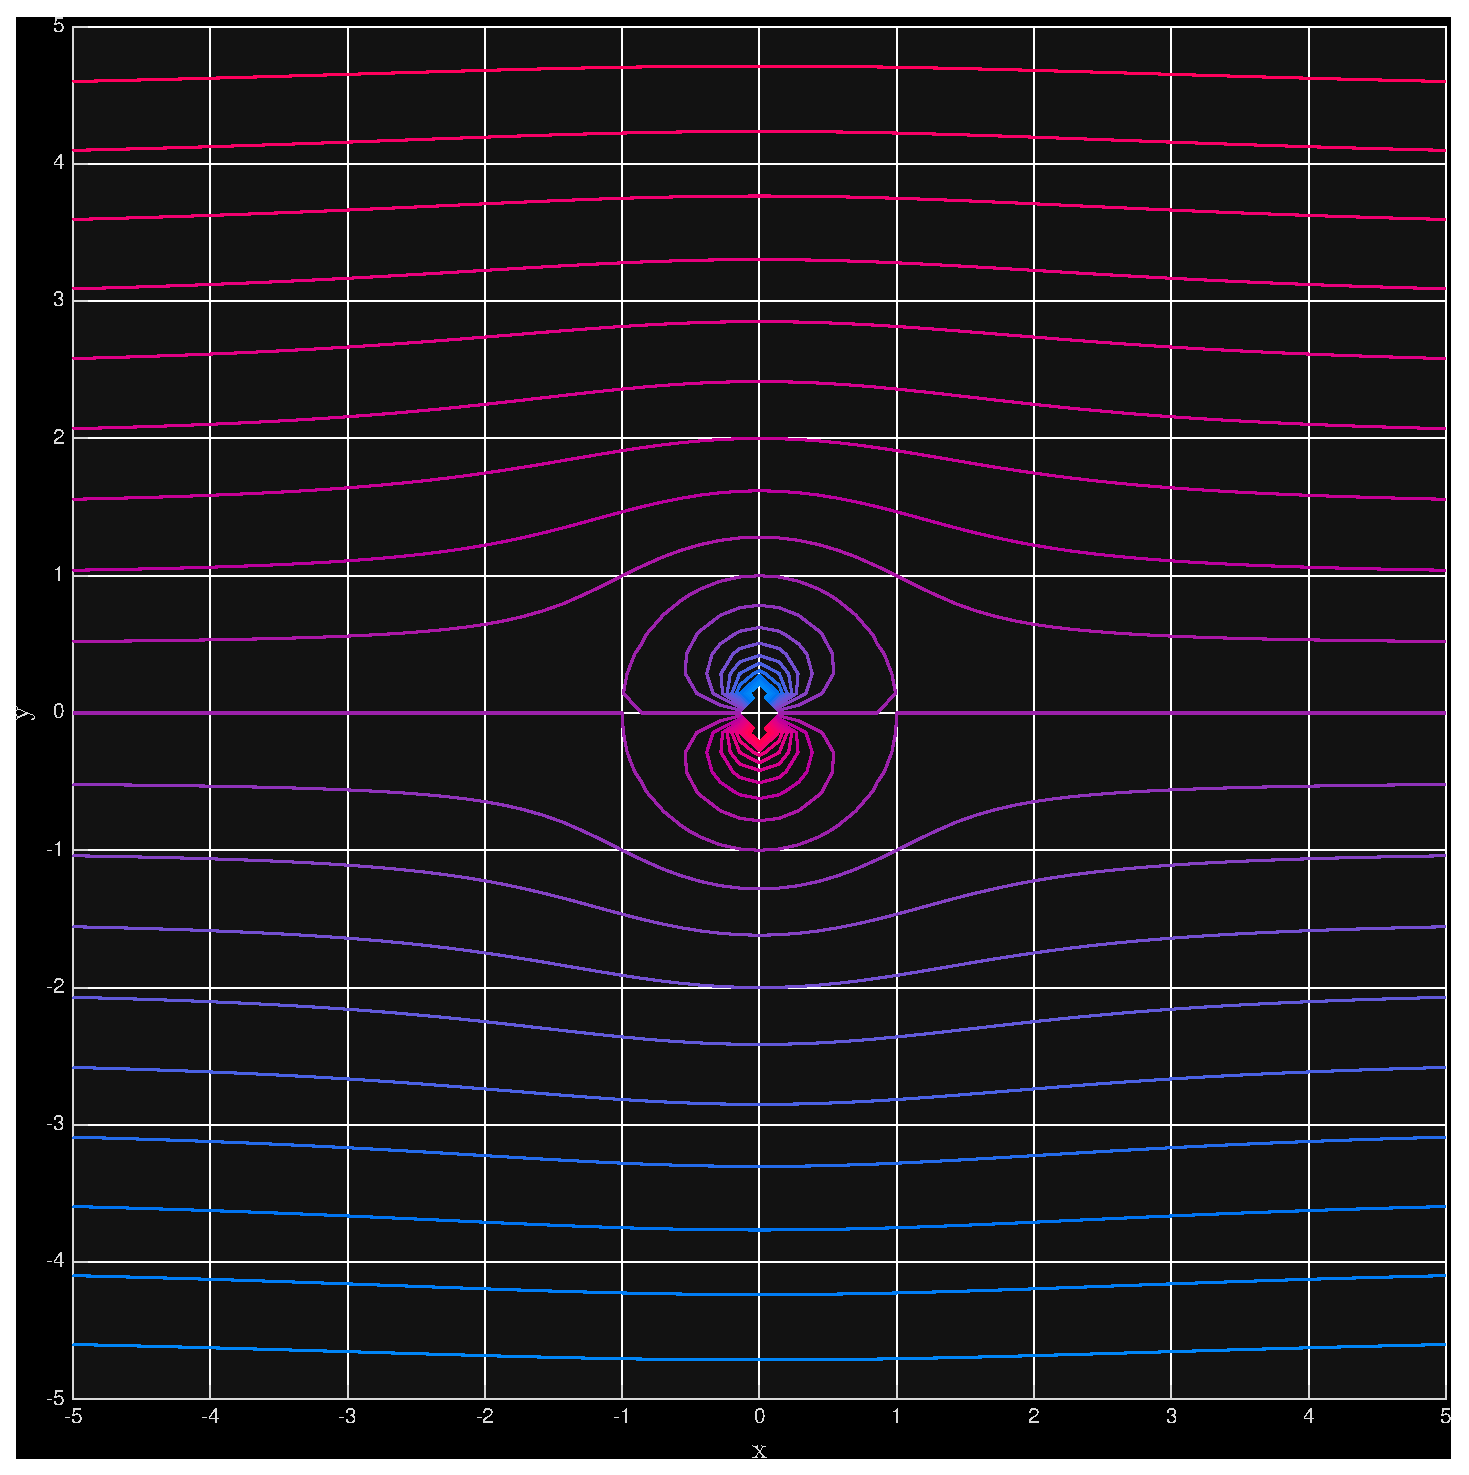
\includegraphics[width=0.8\textwidth]{part4el.eps}
   \caption{Exact Solution}
   \label{ex}
\end{figure}

\clearpage

The final part of this problem asked for flow around an ellipse by leveraging BEMs ability to work around arbitrary geometries.
To do this the polar description of an ellipse was used as follows:

\begin{equation*}
   r(\theta) = \frac{1}{1 - \sqrt{\qty(e\cos(\theta))^2}}, \qquad \text{with} \qquad e = \sqrt{1 - \frac{b^2}{a^2}}
\end{equation*}

\begin{figure}
   \centering
   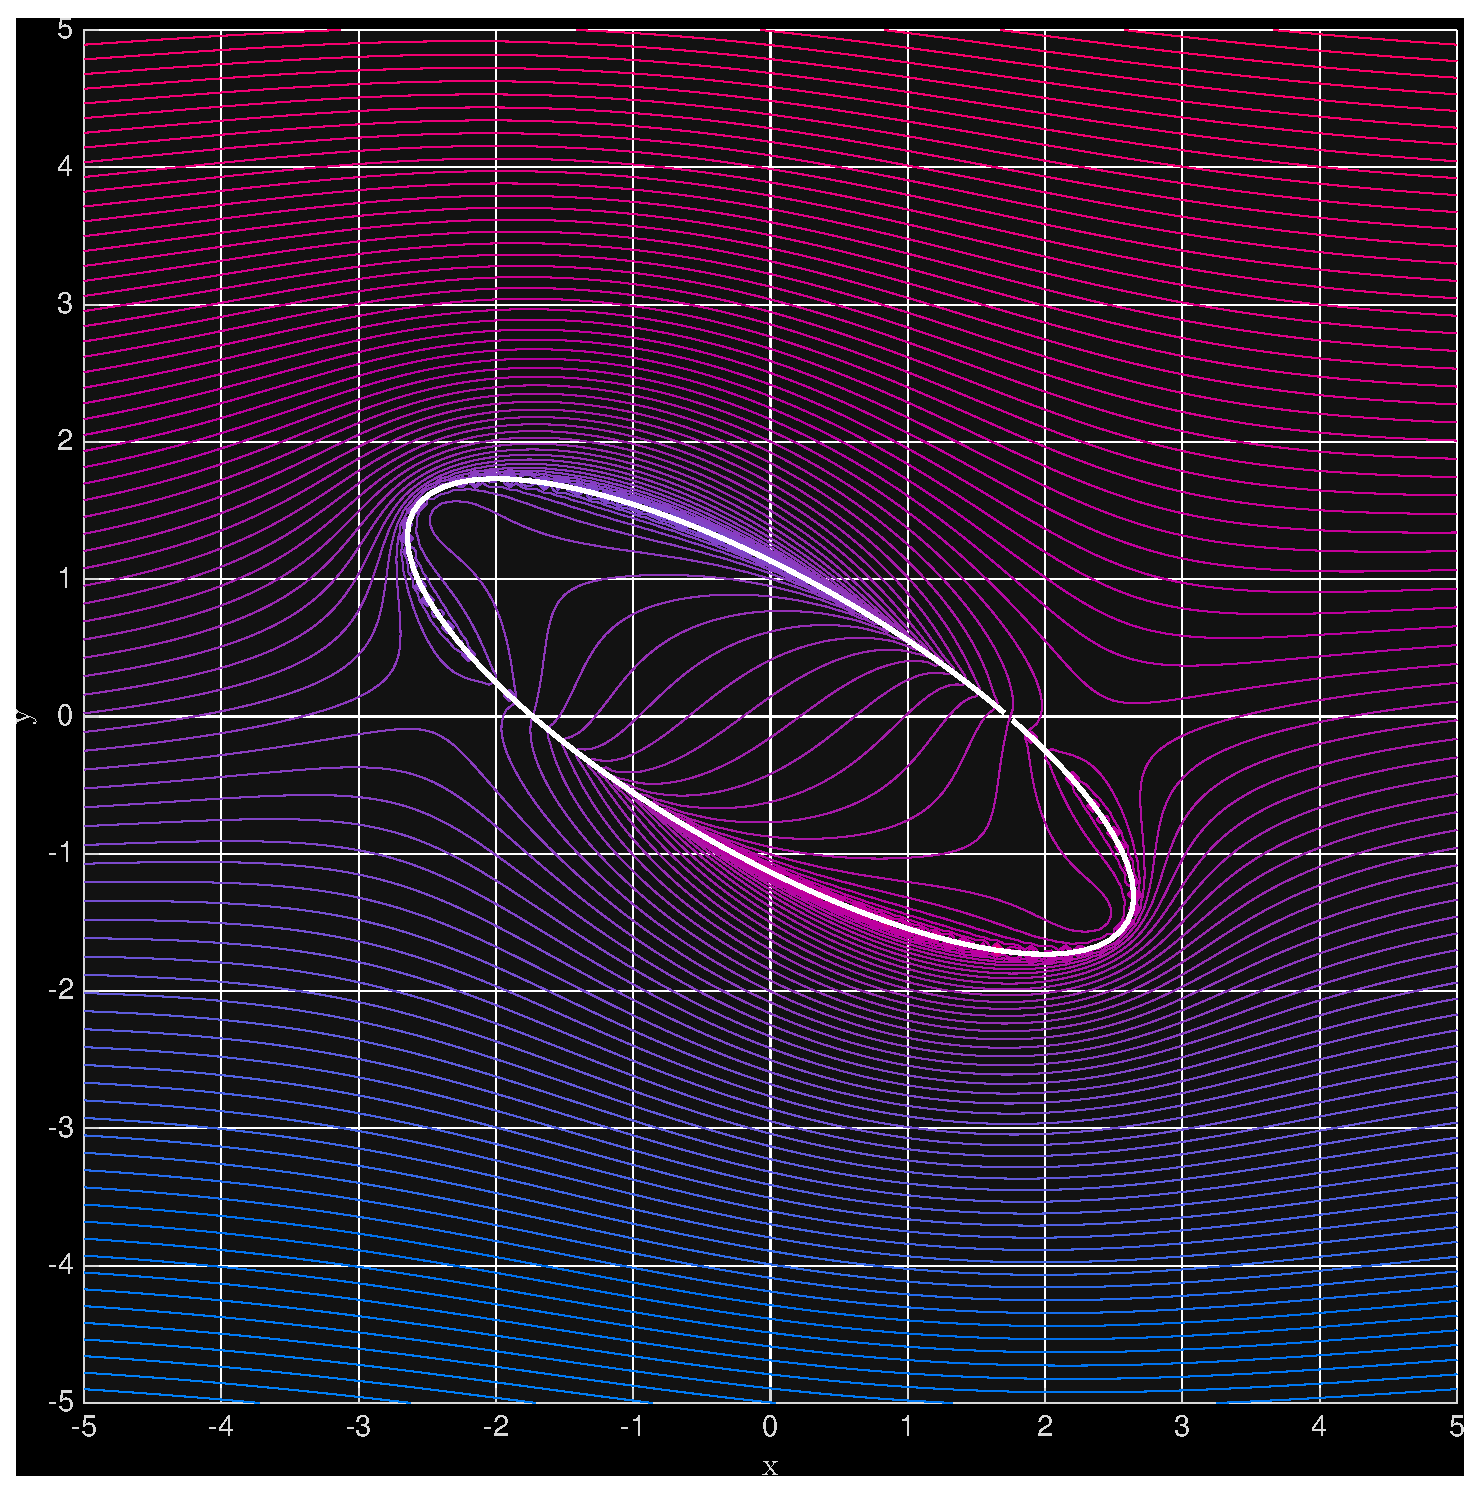
\includegraphics[width=0.8\textwidth]{part3el.eps}
   \caption{3:1 Ellipse, $\alpha$}
   \label{ellipse}
\end{figure}

The boundary can the be set using the relations $x = r\cos(\theta)$ and $y = r\sin(\theta)$ and then most of the method remains the same.
Care needs to be taken with the normal vectors for each panel.
This was done with a simple approximation taking the vector between the two points defining each panel and finding the orthogonal normal vector.
The magnitude of that vector was used for the panel length.

\clearpage

\appendix

\chapter{Analytic Flow}
   \lstinputlisting[language=Matlab,numbers=none]{analytic.m}
\chapter{Cylinder Flow}
   \lstinputlisting[language=Matlab,numbers=none]{laplacian2DCyl.m}
\chapter{Ellipse Flow}
   \lstinputlisting[language=Matlab,numbers=none]{laplacian2DOval.m}
\end{document}
